\documentclass{amsart}
\usepackage[pdftex]{graphicx}
\usepackage{enumerate,placeins}
\graphicspath{{figures/}}

\title{Modeling Intervention Strategies for United States TB Control}
\begin{document}
\maketitle

\section{Abstract}
An extended epidemiological model for Tuberculosis in the US was developed, based on an existing
epidemiological model developed in 2012 by the Centers for Disease Control and Prevention.  
Economic parameters to track the cost burden of TB for the US health care system were added,
and an agent-based stochastic version of the model was implemented.  The sensitivity of the extended
model to changes in parameters was analyzed, and the percentage of foreign-born immigrants with
LTBI appears to be a highly influential parameter in the model.  Intervention strategies to reduce LTBI
among foreign-born arrivals were evaluated, and estimates of the cost per case averted were found.  

\section{Introduction}
Epidemiological models allow public health professionals to predict and analyze
disease dynamics and intervention effectiveness. The most common examples of
such models are compartmental differential equation models, in which the
population is split between several possible health states, with flow between
each state given according to deterministic differential equations. In 2012, 
Hill, Becerra, and Castro implemented a compartmental
differential equaiton model of tuberculosis (TB) in the United States (US).
Their model utilized five health states and two subpopulations, US-born (USB)
and foreign-born (FB) for a total of 10 compartments. They used this model to
evaluate several possible intervention strategies, and ultimately conclude that
though increasing LTBI treatment was a good intervention strategy, the US was
unlikely to meet their stated goal of elimination of TB in the US by 2100. In
this work, the Hill model was extended in several key ways. First, additional
tracking capabilities were added to the Hill model, such that it can now report
further granularity in the disease dynamics. Further, economic components were
added to the model in order to project the US health care system (HCS) costs due
to TB given our current policy as well as for various interventions. Finally, a
population level, agent based implementation of the Hill Model was created, in
order to validate the Hill Model against the natural stochasticity present in
real world disease spread. 

\section{Background}

\subsection{The Hill Model}
A flowchart representation of the Hill Model is shown in Figure 1.  Each compartment
represents a different possible health state with respect to TB for every 
US-born or foreign-born individual, and arrows between different compartments
represent possible transitions between states.  Individuals also leave the model 
from all compartments due to natural death, which is left out of the figure for clarity.  \\

\begin{figure}[h]
  \begin{center}
    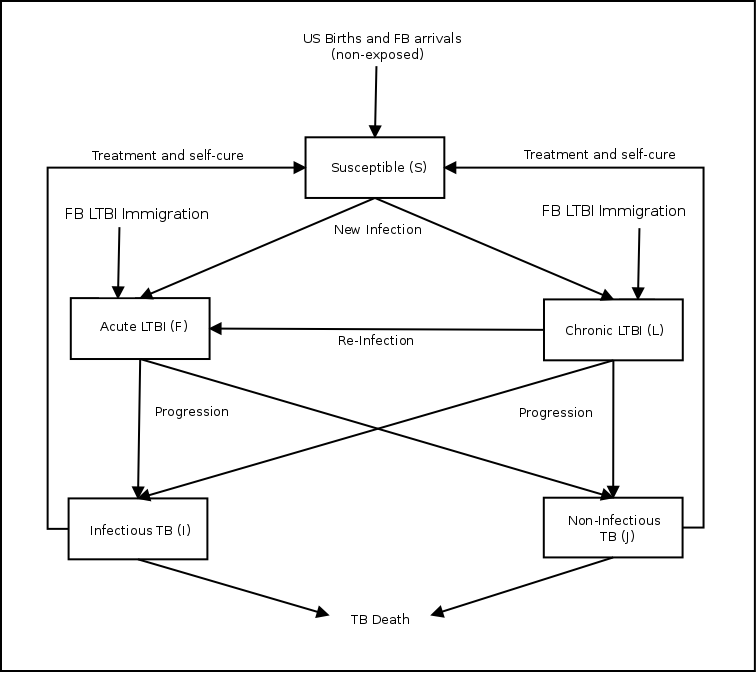
\includegraphics[scale=0.25]{figures/HillModelFlowChart.png}
  \end{center}
  \caption{Schematic of the Hill Model.}
  \label{fig:hillModelSchematic}
\end{figure}

The majority of USB and FB individuals fall into the Susceptible (S) category,
which includes everyone who is uninfected and has not been exposed to TB.  After
exposure to an individual with TB, a person in the Susceptible compartment can
develop Latent TB Infection (LTBI). Latently infected individuals are
asymptomatic and non-infectious, but have some risk of developing active TB
infection over time. To reflect the fact that real LTBI patients have a
much higher risk of developing active TB within two years of exposure, the Hill
Model splits the LTBI compartment into Acute LTBI (fast progressors) and Chronic
LTBI (slow progressors). Accordingly, individuals in the Acute LTBI compartment
have a higher risk of developing active TB than those in the Chronic LTBI
compartment.  Individuals in the Chronic LTBI compartment may also be
exogenously re-infected and transition to the Acute LTBI compartment.  \\

Latently infected individuals may progress to one of two active TB states: Infectious TB (I) or 
Non-Infectious TB (J).  Individuals in both compartments have an increased risk of death from
active TB infection, but only individuals in the Infectious TB compartment are contagious.  
In addition, individuals in all of the infected compartments (F, L, I, J) may be treated or self-cure
themselves of their respective TB health condition.  However, in the model, treatment or self-cure from TB
does not grant immunity, and all healthy individuals are grouped in the Susceptible compartment
and may be re-infected at a later time.  \\

\section{Methods}
\subsection{Basic Structure}
Both the Hill Model (Basic Hill Model) and an extended version of the Hill Model (Extended Hill 
Model) were implemented in 
\texttt{R} as a system of differential equations, which were solved via the
$\texttt{lsoda}$ routine. The systems of differential equations used to capture basic disease dynamics in the Basic Hill Model are shown in Figure 2. In the Extended Hill Model,
more differential equations were implemented to add additional tracking and
economic modeling. These equations are detailed in the Appendix, Section 7.2. 

\begin{figure}
  \begin{center}
    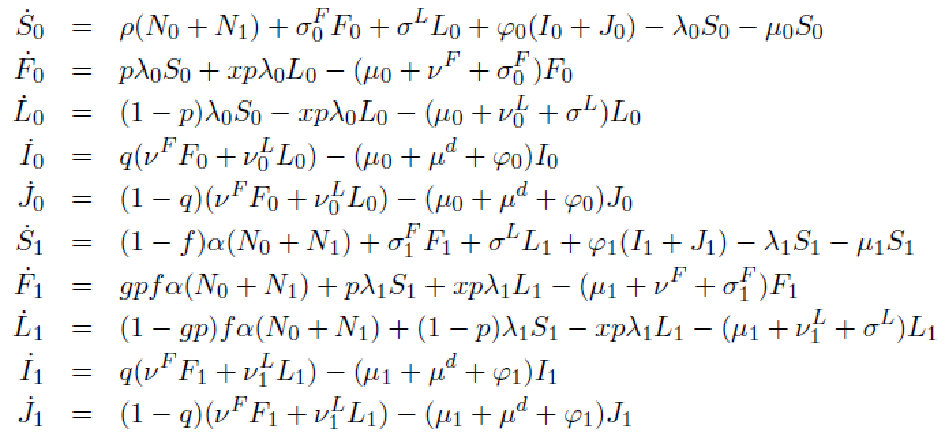
\includegraphics[scale=0.75]{figures/BasicHillEquations.pdf}
  \end{center}
  \caption{System of Differential Equations given in the Hill Model.}
  \label{fig:hillEquations}
\end{figure}

The vector variables $S_{0}, F_{0}, L_{0}, I_{0}, J_{0}$ contain the number of
US-born individuals in the S, F, L, I, J compartments respectively, whereas $S_{1},
F_{1}, L_{1}, I_{1}, J_{1}$ contain foreign-born individuals.  $N_{0}$ and
$N_{1}$ are the total populations of US-born and foreign-born individuals.
The constants $\rho$ and $\alpha$ are birth rates, while $\mu_{i}$, and $\mu_{d}$ are death rates.  
A complete list and descriptions of all constants used in the model can be found in the Appendix,
Section 7.1.

\subsection{Additional Tracking Capabilities}
In order to refine the tracking capabilities of the
Hill Model, the original differential equations used to describe TB spread were
separated into their component parts and each section was tracked separately.
These components were made into compartments, tracked by differential equations
detailed in the appendix. These equations allowed the model to track the total
number of TB cases, TB deaths, and  natural deaths. Further, the model tracks,
the sourced cost on the US HCS. Progressions into
active TB due to activations of LTBI or exogenous infection were tracked,
allowing for sourced incidence data to be generated. The entering cases of LTBI
(acute or chronic) were also tracked. In the case of intervention testing, the
number of cured and untreated cases of entering LTBI were both tracked. Cured
cases of LTBI entering, TB deaths, total TB cases, and total cost were also
tracked discounted at 3\% annually. This discounting was converted to a
continuous differential equation for use within the model. In general, incidence
data is calculated in the same way in the Extended Hill Model as it was in the Basic
Hill Model.

In addition, estimations of the basic reproductive number of FB or USB active,
infectious TB cases were made from a theoretical and an experimental
perspective. Experimental data were calculated by reducing the initial
population of FB or USB active, infectious TB cases by one and allowing the
model to progress otherwise as normal. The decreased number of total TB cases
seen details how many infections can be thought to be due to one infected
individual in the given population.

From an experimental perspective, the spread of TB was thought to be a geometric
series. If one infectious individual infects $x$ people annually, over the
course of $N$ years the total number of infections caused by this individual can
be approximated by the geometric series of $N$ terms with rate $x$ and initial
term $1$. In this case, $N = 100$, and the ratios for FB infectious individuals
and USB infectious individuals were obtained from RATIO CITATION COLIN. 
\subsection{Economic Modeling}
When tracking the economic implications of current US TB load and various
intervention strategies, active TB costs were given by \$14,000. This cost is
the weighted mean of the costs of cases requiring hospitalization (happening
49\% of the time) and cases not requiring hospitalization (51\%). These data
were found in DYLAN COST STUDY CITATION. LTBI treatment costs were given by
\$468.00. These data were based on the cost of a successfull treatment, given by
DYLAN COST STUDY CITATION, as well as adherence and efficacy data found in
ADHERENCE CITATION.

From these estimated cost per treatment, total costs were obtained by assuming
that every patient with active TB in the US is treated at full price, though the
treatment may fail. As individuals with active
TB are charged upon entry to the active TB compartment, the model can also
accurately estimate sourced US HCS cost data. Cost data were separately tracked
due to incoming active TB costs stemming from activation of LTBI vs exogenous
reinfection. These data were modelled as additional compartments and also solved
by $\texttt{lsoda}$. For LTBI treatment cost, treatment was
charged upon leaving the LTBI compartment due to the cumulative self-cure and
treatment rate given in the Hill Model. The fraction of these indviduals who
leave this compartment due to self cure was assumed to be zero. Given the
uncertainty in measurments of LTBI treatment cost, extensive sensitivity
analysis was performed on this parameter relative to final cost outcomes. In
addition to US HCS cost, the system was implemented so as to also track
projected intervention implementation cost, given user-inputted parameters
relating to various possible intervention cost strategies. The extended Hill
Model was used to track the effect of many interventions tested by the Hill
Model. In particular, the intervention strategy of curing entering cases of LTBI
proved very promising and elimination year, final cost, and cost per case
averted were tracked for various levels of entering LTBI cure rate. The
interventions were implemented so as to take effect during the year 2013 and run
to 2100. The numerical DE solver $\texttt{lsoda}$ used was run with a time step
of $0.8$. Sensitivity analysis was performed on this parameter and reducing the
time step was shown to have minimal effect on final size or cost values.

\subsection{Agent Based}
The population level agent based model was implemented in several ways. Early
implementations were built in \texttt{Netlogo} and \texttt{Java}, but final
implementations were constructed in $\texttt{C++}$. An implementation was made
that tracked the hill model exactly, up to still including the Acute Latent
compartment in the model. Probabilites of agent progression between various
health states were computed given rates in the hill model and a variety of
approximations. The model maintained scaled individual records for every
individual with LTBI, with susceptible individuals not modelled as agents.
Instead, a binomial distribution was used to probabilistically pick the number
of new infections each time step. Similarlly, immigration was also handeled
outside of the agent-based modelling. The final size standard deviation and
distribution data was collected via 2160 (MINUS SOME) runs with each agent in
the model truly representing one infected individual and a time step of $0.01$.
These data were analyzed in $R$. This model was also made to track deaths, total
TB cases, and infection sources. This data were consistent with the
deterministic model, and not reproduced in this write-up. 

Further implementations of the \texttt{C++} model were made that deviated from
the basic Hill Model. Specifically, the acute latent compartment in the basic
Hill Model is a vestigal necessity of compartmental modeling and not reflective
of the biology of tuberculosis, and an agent based model was implemented that
more closely respects the biology of tuberculosis. Results from this model or
the strict Hill model did not differ significantly. 
\section{Results}
\subsection{Basic Population Breakdown}
The additional tracking capabilities offered several key insights into US TB
dynamics. Figure~\ref{fig:incPlotSourced} shows the yearly incidence of US TB, broken
down into infection source. It can be seen that the majority of the US TB load
is driven by activations of FB LTBI, followed by USB LTBI activations. This data
further agrees with the conclusions drawn by Hill, Becerra, and Castro about the
necessity of LTBI treatment in any valuable intervention strategy. 
\begin{figure}[h]
  \begin{center}
    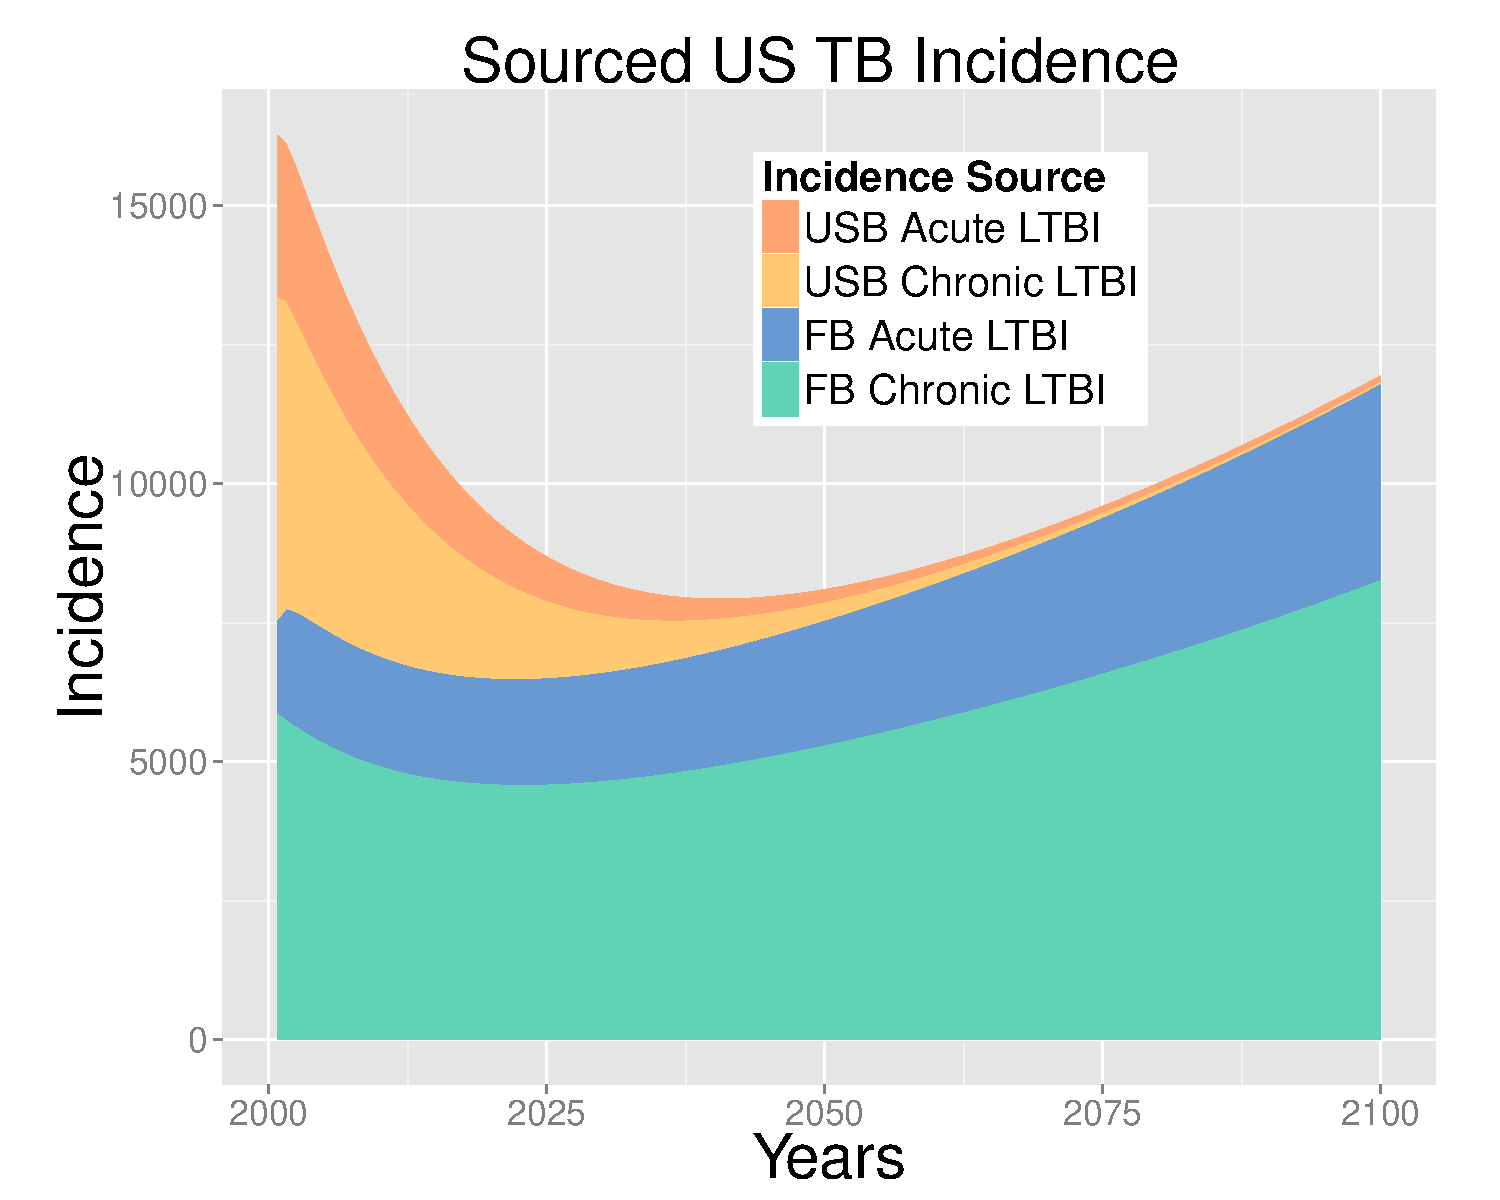
\includegraphics[scale=.5]{incPlotSourced}
  \end{center}
  \caption{Sourced yearly incidence data generated by the extended Hill Model.}
  \label{fig:incPlotSourced}
\end{figure}
Further, figure~\ref{fig:costPlotSourced} shows a similarly sourced plot, but analyzing the
final US HCS costs due to TB. One can see that in this plot, roughly half of the
US TB HCS costs are due to activations of LTBI. In this data, it is appropriate
to think of the costs due to acute LTBI are due to exogenous re-inection,
whereas active TB costs due to chronic LTBI are activations of LTBI into active
TB. 
\begin{figure}[h]
  \begin{center}
    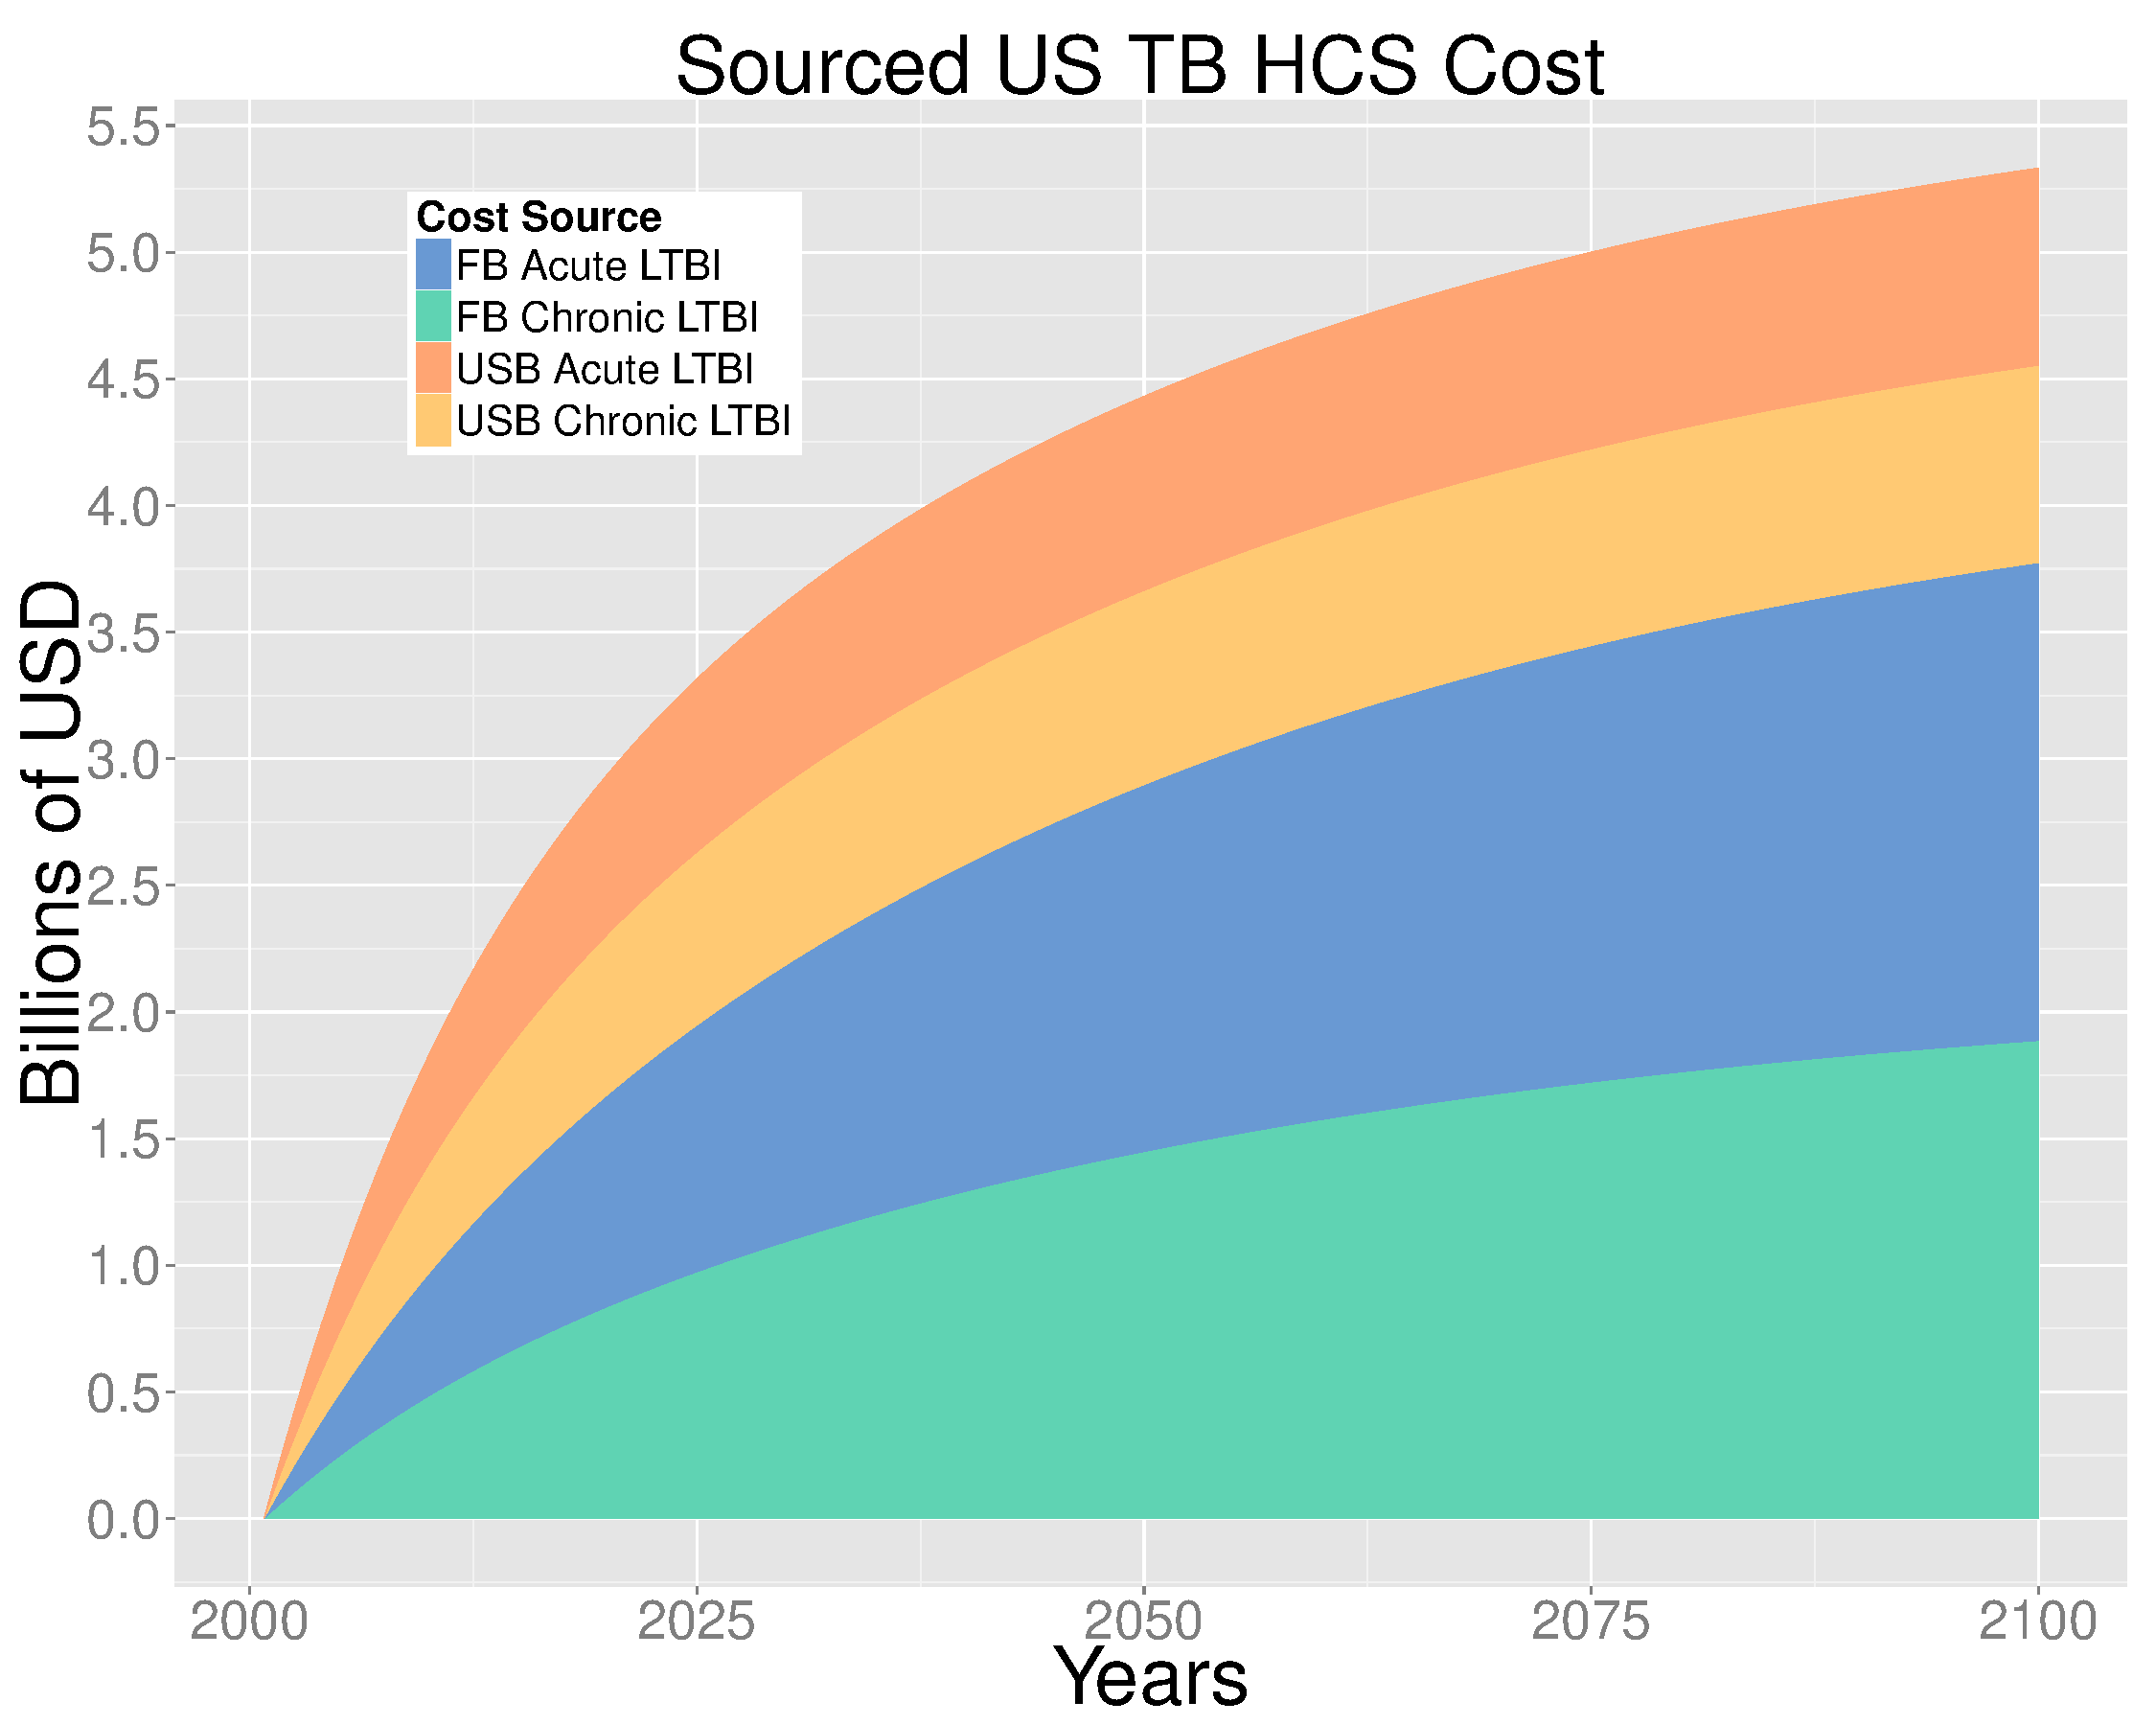
\includegraphics[scale=.35]{costPlotSourced}
  \end{center}
  \caption{Sourced US HCS economic TB load. Note that this data only illustrates
    the load due to treating active TB, but illustrates where the infections
    driving this cost come from.}
  \label{fig:costPlotSourced}
\end{figure}
Note that both of these plots underestimate the impact LTBI activations play in
the spread of TB, as every LTBI activation to infectious TB contributes not only
to incidence and costs directly, but also indirectly by causing additional
future cases, which is not captured in these graphs. Further, there is also US
HCS costs due to treating LTBI, which is not illustrated in these graphs. 
\subsubsection{Basic Reproduction Number}
The basic reproduction number of FB or USB cases of infectious TB was also
estimated by this system. Using the best-fit values of parameters from the 
Hill model, we found the average number of secondary infections arising from
a single case of infectious TB to be 0.423 and 0.370 for USB and FB populations
respectively.  These values differ because in the model, there are different
estimates for death rates and the rate of TB treatment and self-cure in the USB and FB populations, 
so the average infectious period differs between the two populations.
Extrapolating these results, we can think of the
total number of secondary infections over 100 years due to a FB or USB
infectious TB case as describing a geometric series in a large population.
Presuming there are no overlaps in infectious contacts, if a single case of
infectious TB in either population infects $p_f, p_u$ new cases,
respectively, then we can say that over the course of 100 years, the total
number of cases infected will follow a geometric series. This analysis predicts
that over 100 years, one USB infection will lead to $1.04$ subsequent infections,
whereas one FB infection will lead to $.83$ subsequent infections. Experimentally, 
these data were also analyzed, with results of $1.03$ and $.64$, respectively. 
Full calculations are included in the Appendix.  

\subsection{Intervention Analysis}
The primary interventions analyzed by the extended Hill were those that analyzed
curing various percentages of entering LTBI cases. Four indicative percentages
chosen were $5\%$, $10\%$, $25\%$, and $50\%$. Note that the Hill model does
not distinguish documented immigration from undocumented immigration, and as
such estimates of entering LTBI cure rates higher than $50\%$ become much more
difficult to achieve. It was seen that in this model as well as in the basic
Hill, no analyzed intervention predicted elimination by 2100. In order to obtain
elimination by 2100, at least 95\% of entering LTBI cases had to be cured, which
is practically impossible. However, it was seen that curing entering cases of
LTBI resulted in a net US HCS cost per case averted of \$67,654.07 at 2025, \$28,699.15 at 2050,
and \$17,912.95 at 2100 (assuming 25\% reduction with each cure costing \$800; see Table
\ref{tab:cpcaArt} for other percentages). Given the variable nature of LTBI
treatment cost, the model code is extendible such that a user can adjust these
costs themselves to explore more specific methods of curing entering LTBI.
Further, it was also found that the relationship between total incidence at 2100
and percentage of incoming LTBI cases cured was linear, and from this estimates
were made of the yearly average US HCS savings garnered by curing one case of
entering LTBI over the time scale 2000 to 2025, 2000 to 2050, and 2000 to 2100.
This value peaked at \$1.283 billion at 2100 (25\% reduction). This illustrates
that it would be cost saving to cure cases of LTBI at the cost of \$1.283
billion ``2000'' dollars over the time period 2000-2100. These intervention
strategies also resulted in 11,900; 29,880; and 60,189 fewer cases of TB seen in
the US, and 1,025; 2,573; and 5,185 fewer TB deaths, for 10\%, 25\%, and 50\%
reduction, respectively.

% latex table generated in R 3.0.1 by xtable 1.7-1 package
% Mon Oct 14 00:36:15 2013
\begin{table}
\centering
\begin{tabular}{|r|cccc|}
  \hline
 & red5 & red10 & red25 & red50 \\ 
  \hline
2000 & ND & ND & ND & ND \\ 
  2025 & 67908.81 & 67855.46 & 67654.07 & 67332.53 \\ 
  2050 & 28938.23 & 28878.70 & 28699.15 & 28404.13 \\ 
  2075 & 21044.88 & 20989.16 & 20820.53 & 20541.77 \\ 
  2100 & 18130.11 & 18076.11 & 17912.95 & 17642.64 \\ 
   \hline
\end{tabular}
\caption{Cost Per Case Averted by Reducing Incoming LTBI by X percent (in dollar per case)} 
\label{tab:cpcaArt}
\end{table}

Several other intervention strategies analyzed by the Hill Model were refined
with the Extended Hill, and economic properties about each of them were tracked.
The results for these interventions, which are less effective than curing
entering LTBI cases across the board, are given in the appendix. 
\subsection{Agent Based Evaluation}
The Agent Based Model allowed the statistical properties of the system to be
analyzed and verified. In particular, they illustrated that the deterministic
Hill model provides a robust and consistent statistical measure of TB epidemic
behavior in the US conditions. We found that the distribution of incidence and
final population sizes were normal, with mean accurate to the deterministic
model and standard deviations given in table X, in the Appendix. 

\subsection{Sensitivity Analysis}
To account for uncertainty of input parameter values and to gain insight about the
most influential parameters in the model, we used Latin Hypercube Sampling to analyze the deterministic model, implemented with the \texttt{lhs} package in \texttt{R}.  We varied 
the 16 parameters from the original Hill model according to triangular distributions centered
around their best-fit values, and two additional treatment cost parameters according to uniform distributions.  We obtained similar results to the Hill model 
analyzing non-economic outcomes, as expected for validation.  For economic 
outcomes, we found the parameter $f$, the fraction of FB arrivals with LTBI,
to be highly correlated with the projected overall cost burden of TB in the United States
over the next 100 years.  Another highly influential parameter in the model was $\sigma^{L}$, 
the treatment rate for chronic LTBI.  However, while increasing $\sigma^{L}$ significantly
decreases the cost burden due to Active TB treatment, it increases the cost burden due to Latent TB treatment by a greater amount, given the model estimates that Latent TB treament and Active
TB treatment health care costs are approximately \$700 and \$14,000 per case cured respectively.  
A full description of the Latin Hypercube Sampling analysis and tables of Partial Rank Correlation Coefficient (PRCC) results for all parameters are given in the Appendix, Section 7.6.  \\


\section{Discussion}
These results confirm the hypothesis that curing incoming LTBI rates is a
necessary step towards elimination and indicate that it is a cost effective
option. 
\subsection{Future Work}
This work could be extended by examining different classes of interventions or
more accurately estimating intervention cost with the deterministic extended
Hill. Further work could also be done with the agent-based Hill Model, by using
it to examine the effect contact structure plays on US TB incidence levels or to
examine the effects drug-resistant TB will have on US TB dynamics. 
\section{Appendix}
\subsection{Hill Constants}
Below, we detail some of the relevant constants in the Basic Hill Model, and their best-fit
values. A full listing of constants used in the original Hill Model can be found in <CITATION HERE> 
\begin{figure}[h]
  \begin{center}
    \tiny{
    \begin{verbatim}
sigmaLBase  <- 0.057
fBase       <- 0.187
transBase   <- 1
incLTBIBase <- 1


#Treatment Effectiveness Data:
probHosp      <- .49 #Probability of hospitalization for active TB treatment
efficacyLTBI  <- .9  #LTBI treatement efficacy
adherenceLTBI <- .64 #LTBI treatment adherence
probLTBItreatsuccess <- efficacyLTBI*adherenceLTBI 

#Cost Parameter Values: 
costtb   <- 2985   #TB treatment cost w/o hopsitalization <- Dylan supp. p.11-12
costhosp <- 25495  #TB treatment cost w/ hospitalization  <- Dylan supp. p.10
costLTBI <- 403.45 #LTBI treatment cost
Ct       <- costtb*(1-probHosp) + costhosp*probHosp #Cost of active TB treatment
Cl       <- costLTBI/probLTBItreatsuccess           #Cost of LTBI treatment

parms <- c(
mu0   = 1/78,      #Natural mortality rate USB per year
mu1   = 1/53,      #Natural mortality rate FB per year
ro    = 0.018,     #USB birth rate per year
alpha = 0.005,     #FB arrival rate per year
p     = 0.103,     #Fraction of new infections which are acute (fast
progressors)
vF    = 1.5,       #Progression rate of acute infection per year
l0    = 0.015,     #Prevalence of LTBI in the USB population in 2000
l1    = 0.211,     #Prevalence of LTBI in the FB population in 2000: 
r0    = 0.667,     #Fraction of cases due to reactivation in the USB population
r1    = 0.780,     #Fraction of cases due to reactivation in the FB population
vL0   = 0.0014,    #Progression rate for reactivation (chronic LTBI) in the USB
population per year
vL1   = 0.0010,    #Progression rate for reactivation (chronic LTBI) in the FB
population per year
q     = 0.708,     #Fraction of infections progressing to infectious disease
mud   = 0.115,     #Mortality rate due to TB per year
x     = 0.111,     #Fraction of re-infected chronic LTBI moving to acute
infection
ARI0  = 0.030/100, #Annual risk of infection for USB in 2000
beta  = 10.39,     #Effective contact rate per year
e0    = 0.965,     #Fraction of preferred contacts with own population for USB
e1    = 0.985,     #Fraction of preferred contacts with own population for FB
g     = 0.0047,    #Fraction of FB arrivals with LTBI who are fast progressors
phi0  = 1.114,     #Cumulative fraction self-cure and treatment of active
disease for both populations pre year RATES (USB)
phi1  = 1.167,     #Cumulative fraction self-cure and treatment of active
disease for both populations pre year RATES (FB)
sigmaF0 = 1.296,   #Cumulative fraction of treatment for acute infection for
both populations per year RATES (USB)
sigmaF1 = 1.301,   #Cumulative fraction of treatment for acute infection for
both populations per year RATES (FB)
sigmaLBase = sigmaLBase, #Treatment rate for chronic LTBI per year
fBase = fBase,      #Fraction of FB arrivals with LTBI

#2010 New Cases in Population i (millions)
#source: http://www.cdc.gov/mmwr/preview/mmwrhtml/mm5105a3.htm
newCases0 = .008714,  #US-born
newCases1 = .007554,  #Foreign-born

CtBase = Ct,
ClBase = Cl
)
    \end{verbatim}
  }
  \end{center}
  \caption{A list of relevant constants in the Basic \& Extended Hill Model}
  \label{fig:basicHillConstants}
\end{figure}
\subsection{The Extended Hill Equations}
Below, we detail the full equations used in the extended hill model. These
equations extend those used in the standard Hill Model. In many cases, the
equations of the Hill model were split into their component parts, which could
then be tracked separately. 
\begin{figure}[h]
  \begin{center}
  \tiny{
    \begin{verbatim}
discV   <- 1/(1.03^t)  #amount costs, health states discount constant

#parameter values initialized for each time step
c01          <- (1-e0)*((1-e1)*N1)/((1-e0)*N0 + (1-e1)*N1)       #proportion of contacts made with FB individuals  (USB)
c00          <- 1 - c01                                          #proportion of contacts made with USB individuals (USB)
c10          <- (1-e1)*((1-e0)*N0)/((1-e0)*N0 + (1-e1)*N1)       #proportion of contacts made with USB individuals (FB)
c11          <- 1 - c10                                          #proportion of contacts made with FB individuals  (FB)
dLTBIEn      <- f*alpha*(N0+N1)                                  #FB arrivals with LTBI entering
dnatdeath0   <- mu0 * N0                                         #Natural deaths (USB)
dnatdeath1   <- mu1 * N1                                         #Natural deaths (FB)
dtbdeath0    <- mud * (I0 + J0)                                  #TB deaths (USB)
dtbdeath1    <- mud * (I1 + J1)                                  #TB deaths (FB)
dtbdeathD0   <- discV * dtbdeath0                                #TB deaths with discounting (USB)
dtbdeathD1   <- discV * dtbdeath1                                #TB deaths with discounting (FB)
dprogAcute0  <- vF*F0                                            #Acute LTBI progressions to Active TB disease (USB)
dprogAcute1  <- vF*F1                                            #Acute LTBI progressions to Active TB disease (FB)
dprogChron0  <- vL0*L0                                           #Chronic LTBI progressions to Active TB disease (USB)
dprogChron1  <- vL1*L1                                           #Chronic LTBI progressions to Active TB disease (FB)
dprogTotal0  <- dprogAcute0 + dprogChron0                        #Progression to Active TB (USB)
dprogTotal1  <- dprogAcute1 + dprogChron1                        #Progression to Active TB (FB)
dprogTotalD0 <- discV * dprogTotal0                              #Progression to Active TB with discounting (USB)
dprogTotalD1 <- discV * dprogTotal1                              #Progression to Active TB with discounting (FB)
lambda0      <- transmission*(beta*(c00*(I0/N0) + c01*(I1/N1)))  #Forces of Infection (USB)
lambda1      <- transmission*(beta*(c10*(I0/N0) + c11*(I1/N1)))  #Forces of Infection (FB)
dexogenous0	 <- x*p*lambda0*L0                                   #Exogenous re-infections of Chronic LTBI to Acute LTBI (USB)
dexogenous1  <- x*p*lambda1*L1                                   #Exogenous re-infections of Chronic LTBI to Acute LTBI (FB)
dInterventionCost <- discV * (iCnewCases*1e6*(dprogTotal0+dprogTotal1) + iCtotPop*1e6*(N0+N1) + iCLTBIEn*1e6*dLTBIEn*(1-incLTBI))

#Difference Equations (USB)
dS0 <- ro*(N0+N1) + sigmaF0*F0 + sigmaL*L0 + phi0*(I0+J0) - lambda0*S0 - mu0*S0
dF0 <- p*lambda0*S0 + dexogenous0 - (mu0 + vF + sigmaF0)*F0
dL0 <- (1-p)*lambda0*S0 - dexogenous0 - (mu0 + vL0 + sigmaL)*L0
dI0 <- q*(dprogAcute0 + dprogChron0) - (mu0 + mud + phi0)*I0
dJ0 <- (1-q)*(dprogAcute0 + dprogChron0) - (mu0 + mud + phi0)*J0

#Difference Equations (FB)
dS1 <- (1-incLTBI)*dLTBIEn+(1-f)*alpha*(N0+N1) + sigmaF1*F1 + sigmaL*L1 + phi1*(I1 + J1) - lambda1*S1 - mu1*S1
dF1 <- g*p*dLTBIEn*incLTBI + p*lambda1*S1 + dexogenous1 - (mu1 + vF + sigmaF1)*F1
dL1 <- (1-g*p)*dLTBIEn*incLTBI + (1-p)*lambda1*S1 - dexogenous1 - (mu1 + vL1 +sigmaL)*L1
dI1 <- q*(dprogAcute1 + dprogChron1) - (mu1 + mud + phi1)*I1
dJ1 <- (1-q)*(dprogAcute1 + dprogChron1) - (mu1 + mud + phi1)*J1

dN0 <- dS0 + dF0 + dL0 + dI0 + dJ0
dN1 <- dS1 + dF1 + dL1 + dI1 + dJ1

#Cost calculations
dcL0 <- discV * Cl * sigmaL  * 1e6 * L0                    #cost for Chronic LTBI cures      (USB)
dcF0 <- discV * Cl * sigmaF0 * 1e6 * F0                    #cost for Acute LTBI cures        (USB)
dcI0 <- discV * Ct * q*(dprogAcute0 + dprogChron0) * 1e6     #cost for Infectious TB cures     (USB)
dcJ0 <- discV * Ct * (1-q)*(dprogAcute0 + dprogChron0) * 1e6 #cost for Non-Infectious TB cures (USB)
dcI0dL0 <- discV * Ct * q*(dprogChron0) * 1e6     #cost for Infectious TB cures     (USB)
dcI0dF0 <- discV * Ct * q*(dprogChron0) * 1e6     #cost for Infectious TB cures     (USB)
dcJ0dL0 <- discV * Ct * (1-q)*(dprogAcute0) * 1e6 #cost for Non-Infectious TB cures (USB)
dcJ0dF0 <- discV * Ct * (1-q)*(dprogAcute0) * 1e6 #cost for Non-Infectious TB cures (USB)
dcL1 <- discV * Cl * sigmaL  * 1e6 * L1                    #cost for Chronic LTBI cures      (FB)
dcF1 <- discV * Cl * sigmaF1 * 1e6 * F1                    #cost for Acute LTBI cures        (FB)
dcI1 <- discV * Ct * q*(dprogAcute1 + dprogChron1) * 1e6     #cost for Infectious TB cures     (FB)
dcJ1 <- discV * Ct * (1-q)*(dprogAcute1 + dprogChron1) * 1e6 #cost for Non-Infectious TB cures (FB)
dcI1dL1 <- discV * Ct * q*(dprogChron1) * 1e6     #cost for Infectious TB cures     (USB)
dcI1dF1 <- discV * Ct * q*(dprogChron1) * 1e6     #cost for Infectious TB cures     (USB)
dcJ1dL1 <- discV * Ct * (1-q)*(dprogAcute1) * 1e6 #cost for Non-Infectious TB cures (USB)
dcJ1dF1 <- discV * Ct * (1-q)*(dprogAcute1) * 1e6 #cost for Non-Infectious TB cures (USB)
dcN0 <- dcF0 + dcL0 + dcI0 + dcJ0                            #Total cost for all treatments (USB)
dcN1 <- dcF1 + dcL1 + dcI1 + dcJ1                            #Total cost for all treatments (FB)
    \end{verbatim}
  }
  \end{center}
  \label{fig:extendedHillEqs}
  \caption{
    The equations defining the Extended Hill Model, shown in \texttt{R} syntax.
    In this model, compartments share the same names as they did in the Hill
    Model, \emph{i.e.} \texttt{S1} is the Foreign Born susceptible population. 
  }
\end{figure}
Here, a continuous discounting approximation is used to a discount rate of $3\%$
yearly, found via $discV$. In many of the differential equations, a small $c$ is
used to denote \emph{cost of}. 
\FloatBarrier
\subsection{Estimations for Infectious Rates of FB and USB}

\subsection{Statistical Qualities of the Agent Based Model}
\subsection{Finer Intervention Analysis}

% latex table generated in R 3.0.1 by xtable 1.7-1 package
% Mon Oct 14 00:36:15 2013
\begin{table}
\centering
\begin{tabular}{|r|cccc|}
  \hline
 & red5 & red10 & red25 & red50 \\ 
  \hline
2000 & 0.00 & 0.00 & 0.00 & 0.00 \\ 
  2025 & 1115.12 & 2231.70 & 5592.43 & 11227.57 \\ 
  2050 & 3406.41 & 6821.27 & 17117.18 & 34447.71 \\ 
  2075 & 4976.77 & 9967.15 & 25021.33 & 50389.58 \\ 
  2100 & 5942.02 & 11900.90 & 29880.03 & 60189.49 \\ 
   \hline
\end{tabular}
\caption{Cases of TB Averted by Reducing Incoming LTBI by X percent (Cure=\$800)} 
\label{tab:caRed}
\end{table}

% latex table generated in R 3.0.1 by xtable 1.7-1 package
% Mon Oct 14 00:36:15 2013
\begin{table}
\centering
\begin{tabular}{|r|cccc|}
  \hline
 & red5 & red10 & red25 & red50 \\ 
  \hline
2000 & ND & ND & ND & ND \\ 
  2025 & 67908.81 & 67855.46 & 67654.07 & 67332.53 \\ 
  2050 & 28938.23 & 28878.70 & 28699.15 & 28404.13 \\ 
  2075 & 21044.88 & 20989.16 & 20820.53 & 20541.77 \\ 
  2100 & 18130.11 & 18076.11 & 17912.95 & 17642.64 \\ 
   \hline
\end{tabular}
\caption{Cost Per Case Averted by Reducing Incoming LTBI by X percent (in dollar per case, Cure=\$800)} 
\label{tab:cpcaRed}
\end{table}

\subsection{Latin Hypercube Sampling}
The model parameters and variable names referred to in this analysis are listed below, along with best-fit or estimated values.  Following the example of the Hill model, we generated a Latin Hypercube Sample varying 18 of the input parameters.  From these parameters, 16 are identical to the input parameters varied in the sensitivity analysis of the original Hill model, and the remaining two parameters, $C_{A}$ and $C_{L}$, are variables for the average cost of Active and Latent TB treatment in the US.   Probability distributions for the original 16 parameters of the Hill model were all set to be Triangular, with mode at the best fit value and end points at the 2.5 and 97.5 percentile values reported in the Hill model.  Probability distributions for $C_{A}$ and $C_{L}$ were set to be Uniform, with range +/- 10\% of the estimated value.  All probabilty distributions used to generate the Latin Hypercube are listed in Table 1.\\

\vspace{5mm}
{\bf Original Hill Model Parameters} 
(USB = US born, FB = Foriegn born)
\begin{enumerate}[1.] \itemsep 0em
\item{$\sigma^{L}$ = 0.057 (Treatment rate for chronic LTBI)}
\item{$v^{L}_{0}$   = 0.0014 (Progression rate for reactivation in the USB population)}
\item{$v^{L}_{1}$  = 0.0010 (Progression rate for reactivation in the FB population)}
\item{$f$                = 0.187 (Fraction of FB arrivals with LTBI)}
\item{$p$               = 0.103 (Fraction of new infections which are acute)}
\item{$ARI_{0}$     = 0.00030 (2000 Annual Risk of Infection, USB)}
\item{$q$               = 0.708 (Fraction of infections progressing to infectious disease)}
\item{$g$               = 0.0047 (Fraction of FB arrivals with LTBI who are fast progressors)}
\item{$\sigma^{F}$ = 0.461 (Cumulative fraction of treatment for acute infection)}
\item{$r_{0}$          = 0.667 (Fraction of cases due to reactivation in USB population)}
\item{$r_{1}$          = 0.780 (Fraction of cases due to reactivation in FB population)}
\item{$\mu^{d}$      = 0.115 (Mortality rate due to TB)}
\item{$x$                 = 0.111 (Fraction of re-infected chronic LTBI moving to acute infection)}
\item{$\phi$            = 0.897 (Cumulative fraction self-cure and treatment of active disease)}
\item{$e_{0}$          = 0.965 (Fraction of preferred contacts within own population for USB)}
\item{$e_{1}$          = 0.985 (Fraction of preferred contacts within own population for FB)}
\end{enumerate}
\vspace{2mm}
{\bf Additional Cost Parameters}
\begin{enumerate}[1.] \itemsep 0em
\item{$C_{A}$           = \$14,014.50 (Cost per Active TB treatment)}
\item{$C_{L}$           = \$700 (Cost per Latent TB treatment)}
\end{enumerate}
\vspace{5mm}

\begin{table}[h]
\centering
\begin{tabular}{l l}
\hline\hline\\
Parameter & Distribution\\ [0.5ex]
\hline\\
$\sigma_{L}$  & Tri(0.015,0.057,0.086) \\
$v^{L}_{1}$   & Tri(0.0009,0.0010,0.0014) \\
$f$                 & Tri(0.157,0.187,0.232) \\
$p$                & Tri(0.053,0.103,0.137) \\
$ARI_{0}$      & Tri(0.00021,0.00030,0.00030) \\
$q$                & Tri(0.569,0.708,0.825) \\
$g$                & Tri(0.0008,0.0047,0.0815)  \\
$\sigma_{F}$ & Tri(0.419,0.461,0.574) \\
$r_{1}$          & Tri(0.759,0.780,0.831) \\
$r_{0}$          & Tri(0.623,0.667,0.694) \\
$\mu^{d}$      & Tri(0.071,0.115,0.231) \\
$x$                 & Tri(0.088,0.111,0.860) \\
$v^{L}_{0}$   & Tri(0.0011,0.0014,0.0015) \\
$\phi$            & Tri(0.861,0.897,0.938) \\
$e_{0}$          & Tri(0.853,0.965,0.995) \\
$e_{1}$          & Tri(0.877,0.985,0.999) \\
$C_{A}$           & Uniform(12613,15416) \\
$C_{L}$           & Uniform(630,770) \\ [1ex]
\hline
\end{tabular}\\[1ex]

{\bf Table 1.} Probability distributions for model parameters, where Tri(x,y,z) denotes the 
Triangular distribution with endpoints (x,z) and mode y.
\end{table}

With a random Latin Hypercube Sample of size n=100,000, we computed partial rank correlation coefficients (PRCC) for each of the initial parameters and treatment costs, according to four different outcomes: 1) projected annual incidence in 2100 in the overall population, 2) projected cumulative cost of Latent TB treatments by 2100, 3) projected cumulative cost of Active TB treatments by 2100, 4) projected cumulative total cost of TB treatments by 2100.  For outcome 1, PRCC values are shown alongside PRCC values computed in the original Hill model for the same outcome in Table 2, showing the closeness of our findings to the sensitivity results of the original Hill model.  PRCC values for the remaining outcomes are reported in Table 3.  \\

\begin{table}[h]
\centering
\begin{tabular}{l r r}
\hline\hline\\
Parameter & Extended Hill Model & Original Hill model \\ [0.5ex]
\hline\\
$\sigma^{L}$  & -0.9303 & -0.9381 \\
$v^{L}_{1}$   & 0.7871  & 0.8309 \\
$f$                 & 0.7050  & 0.8072 \\
$p$                & 0.8369  & 0.6100 \\
$ARI_{0}$      & 0.5950  & 0.4939 \\
$q$                & 0.5797  & 0.4543 \\
$g$                & 0.6122  & 0.4517 \\
$\sigma^{F}$ & -0.4911 & -0.3772 \\
$r_{1}$          & 0.0028  & -0.1109 \\
$r_{0}$          & 0.0018  & 0.0760 \\
$\mu^{d}$      & 0.0923 & 0.0513 \\
$x$                 & 0.0999 & 0.0345 \\
$v^{L}_{0}$    & 0.0133 & 0.0266 \\
$\phi$             & 0.0082 & 0.0177 \\
$e_{0}$          & 0.0178 & -0.0072 \\
$e_{1}$          & 0.1154 & 0.0046 \\
$C_{A}$          & -0.0023 & N/A \\
$C_{L}$           & 0.0009 & N/A \\ [1ex]
\hline
\end{tabular}\\[1ex]

{\bf Table 2.} PRCC values for projected annual incidence in 2100
 in the overall population, alongside corresponding values from the
original Hill model.
\end{table}

From Table 2, we see that the PRCC values in the Extended Hill Model and the Original Hill Model match up reasonably well.  In both cases, $\sigma^{L}$ is the most influential parameter, with PRCC values around -0.93.  The cost parameters $C_{A}$ and $C_{L}$ have PRCC values close to zero, which is expected because varying the treatment costs should not affect the incidence rate of TB.  Parameters in the original Hill model with small PRCC magnitudes (less than 0.15) also have small PRCC values in the extended model, while parameters with larger PRCC magnitudes (greater than 0.35) similarly have large PRCC values in the extended model.  This validates the non-economic components of our model against the original Hill model.   \\

\begin{table}[h]
\centering
\begin{tabular}{l r r r}
\hline\hline\\
Parameter & Latent Costs & Active Costs & Total Costs\\ [0.5ex]
\hline\\
$\sigma^{L}$  & 0.9612  & -0.9284 & 0.4169 \\
$v^{L}_{1}$   & -0.4190 & 0.6470  & 0.3533 \\
$f$                 & 0.7467  & 0.5493  & 0.8083 \\
$p$                & 0.3371  & 0.8810  & 0.8776 \\
$ARI_{0}$      & 0.3920  & 0.6728  & 0.7337 \\
$q$                & 0.3837  & 0.6573  & 0.7200 \\
$g$                & 0.1120  & 0.5369  & 0.5182 \\
$\sigma^{F}$ & -0.1138 & -0.5631 &-0.5435 \\
$r_{1}$          & 0.1253 &  0.0658  & 0.1401 \\
$r_{0}$          & 0.1325  & 0.0878  & 0.1658 \\
$\mu_{d}$      & 0.0249 & 0.0560  & 0.0613 \\
$x$                 & 0.0214 & 0.1282  & 0.1253 \\
$v^{L}_{0}$   & -0.3103 & 0.0502  &-0.1867 \\
$\phi$            & -0.0023 & -0.0102 &-0.0107 \\
$e_{0}$          & 0.0081 & 0.0253   & 0.0269 \\
$e_{1}$          & 0.0804 & 0.1653   & 0.1926 \\
$C_{A}$          & 0.0011 & 0.7024   & 0.6385 \\
$C_{L}$           & 0.8515 & 0.0013  & 0.7598 \\ [1ex]
\hline
\end{tabular}\\[1ex]

{\bf Table 3.} PRCC values for cumulative US Health Care system costs from 
Latent TB treatment, Active TB treatment, and Total treatment costs
\end{table}

In Table 3, we see that the cost parameters $C_{A}$ and $C_{L}$ are highly correlated with Active treatment costs and Latent treatment costs respectively.  These high PRCC values are expected because there is a linear relationship between $C_{A}$ and the cumulative Active treatment cost, and similarly for $C_{L}$ and the cumulative Latent treatment cost.  In addition, we note that both $C_{A}$ and $C_{L}$ are influential in the total overall cost, with PRCC values of 0.6385 and 0.7598 respectively.  Because the PRCC value for $C_{L}$ is greater here, despite the fact that $C_{A} > C_{L}$, we can infer that cumulative Latent TB treatment costs are projected to be greater than cumulative Active TB costs with these estimates for cost parameters, so $C_{L}$ is a more influential parameter for total cumulative treatment costs.  \\

Other variables with significant PRCC magnitudes (greater than 0.5) in Table 3 include $\sigma^{L}$, $v^{L}_{1}$, $f$, $p$, $ARI_{0}$, $q$, $g$, and $\sigma^{F}$.  Two of these parameters, $\sigma^{L}$ and $v^{L}_{1}$, have relatively large PRCC magnitudes for both Latent and Active Costs, but smaller PRCC magnitudes for Total Costs.  Because their PRCC values for each of these two outcomes is different in sign, the net change to the total cost is partially cancelled out, so these parameters have a reduced influence on final US healthcare system costs.  On the other hand, parameters such as $f$ and $p$ have large positive PRCC values for both Latent Costs and Active Costs, and we observe large positive PRCC values for Total Costs as well.\\

To gain insight about strategies to reduce the cost burden for TB in the US, we focus on the parameters with the greatest PRCC magnitudes for Total Cost aside from $C_{A}$ and $C_{L}$, namely $f$, $p$, $ARI_{0}$, and $q$.  All these parameters have PRCC magnitudes above 0.7, and are highly correlated with the total cost burden of TB borne by the US projected over the next 100 years.  Out of these, $ARI_{0}$ is based on a historical fixed value, the Annual Risk of Infection among the US born population in the year 2000, and therefore is unchangeable under any intervention strategy.  The parameters $p$ (the fraction of new infections which are acute) and $q$ (the fraction of infections progressing to infectious disease) are variables which depend on physiological disease dynamics, and may be altered with advances in medicine or mutations in the bacterial strains of TB.  The parameter $f$ is the fraction of FB arrivals with LTBI, which may vary depending on US immigration policies and medical practices.  These results suggest that treating cases of LTBI among new FB arrivals may be the most cost efficient intervention strategy to reduce the disease burden for TB in the US, under the assumptions of the Hill model.  \\

\subsection{Stochastic Model}

\end{document}
